\section{Experimental Apparatus}\label{sec:app}

We designed a compressed air network in a laboratory environment with various leak and pressure conditions to mimic real world challenges and perform experiments under controlled conditions. 
This system was used to develop the dataset for compressed air leak detection using audible sound, discussed in Section \ref{sec:dataset}.
To simulate a real factory setting, the experimental system also includes a speaker system to play background noise from real production facilities while leak sounds are being recorded.
To evaluate the effect of microphone positions, the data is recorded using microphones placed at different distances and orientations from the leak source.

\subsection{Compressed Air System}\label{subsec:app}

\begin{figure}[h]
	\centering
    \begin{subfigure}[t]{0.48\columnwidth}
        \centering
        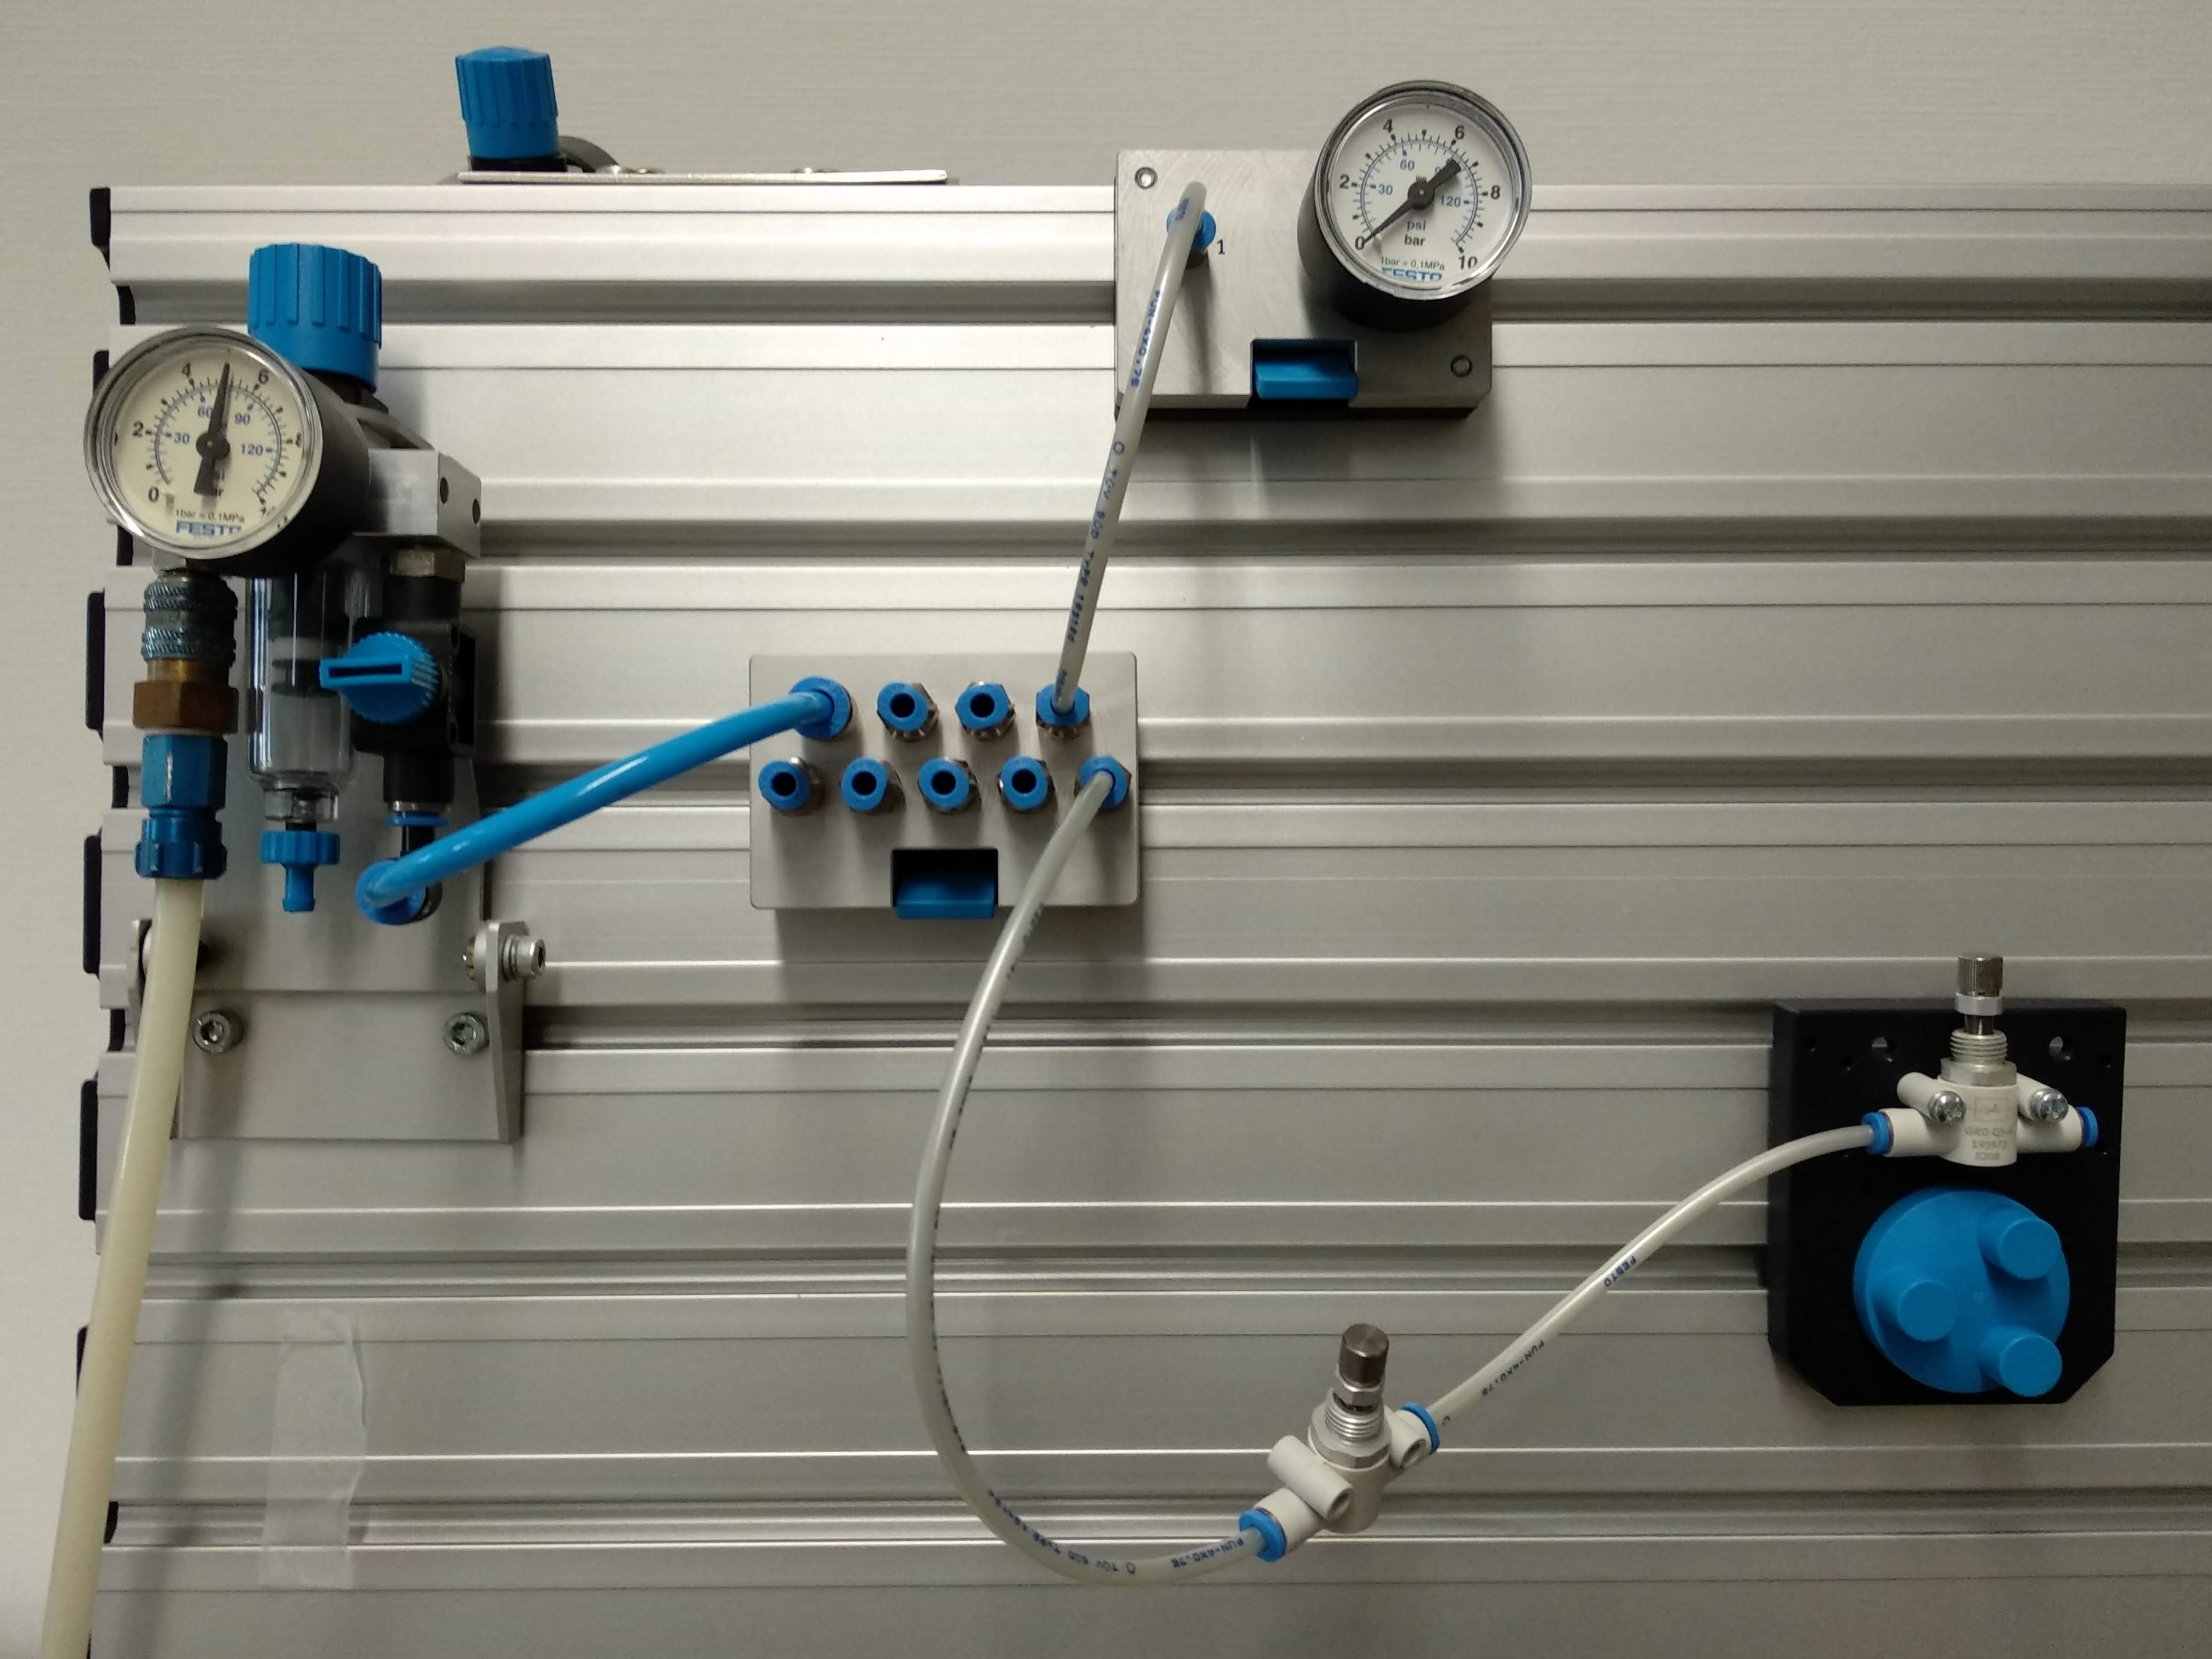
\includegraphics[width=\columnwidth]{images/apparatus_front.jpg}
        \caption{Front view}
        \label{fig:sys-front}
    \end{subfigure}%
    ~ 
    \begin{subfigure}[t]{0.48\columnwidth}
        \centering
        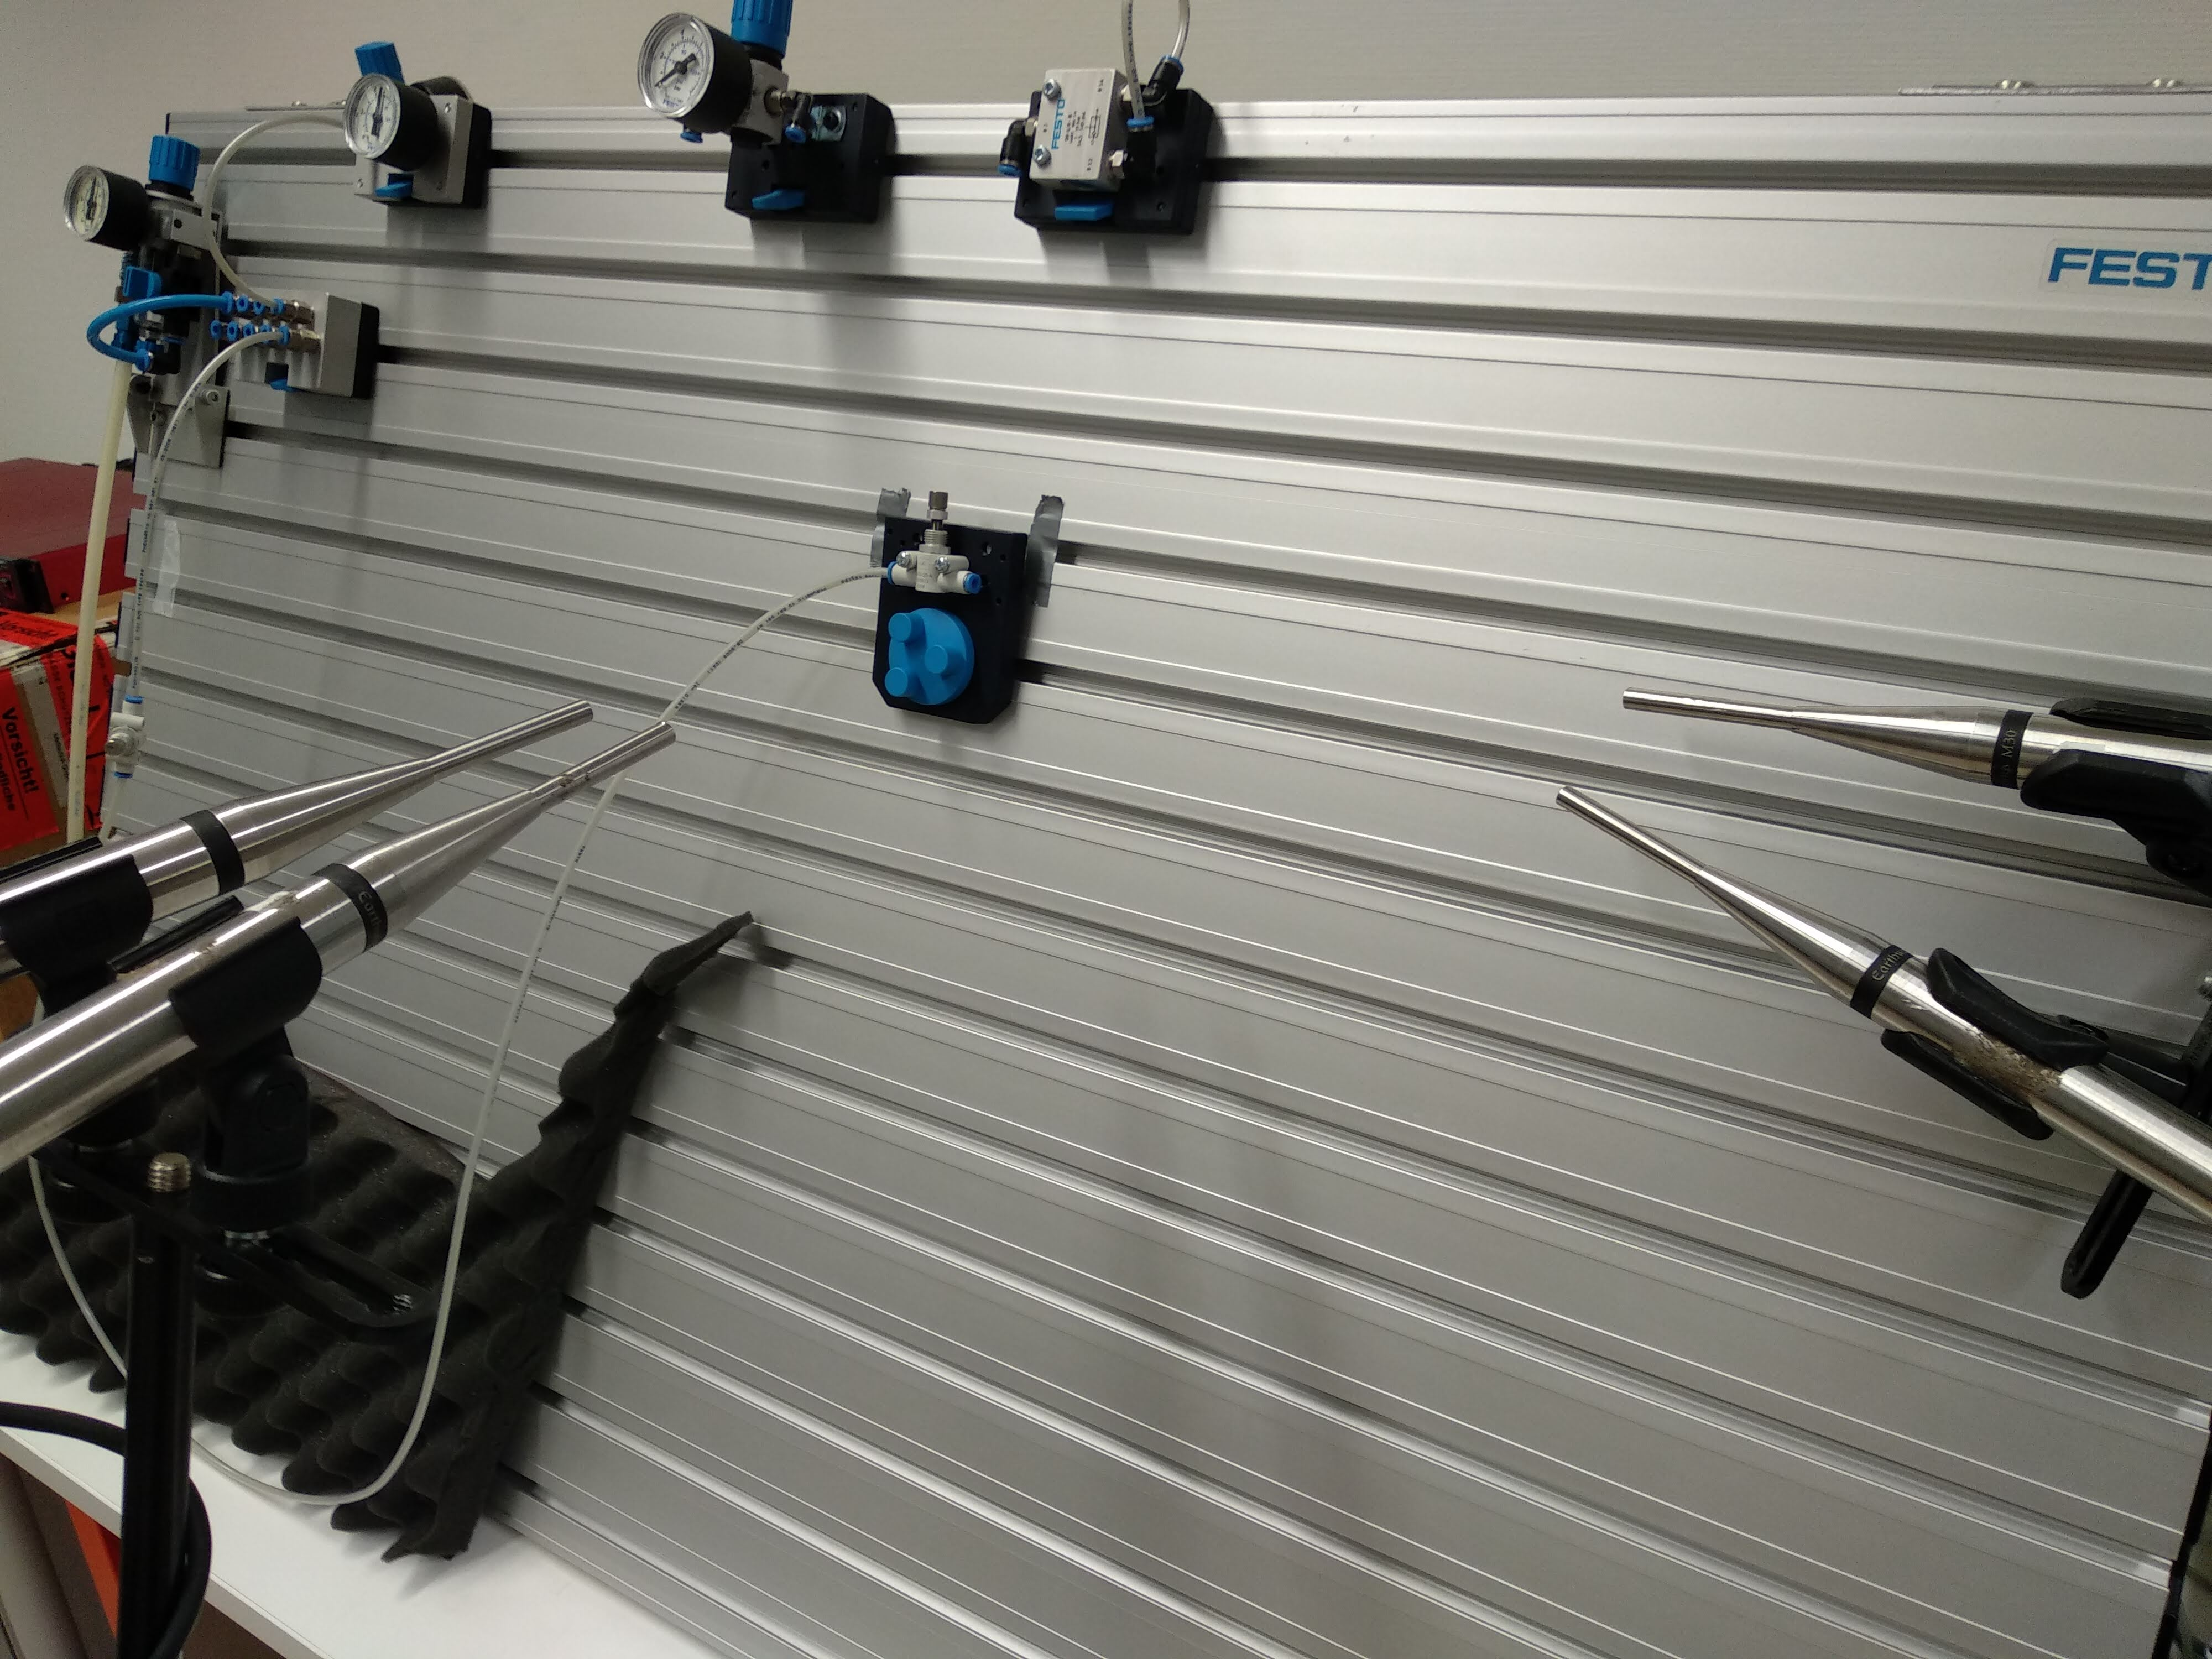
\includegraphics[width=\columnwidth]{images/apparatus_side_angle.jpg}
        \caption{Side view including microphones}
        \label{fig:sys-side}
    \end{subfigure}
	\caption{Experimental apparatus for compressed air leakage data acquisition.}
	\label{fig:sys}
\end{figure}

The experimental apparatus used for data acquisition was developed using a Festo Didactic system\footnote{\url{https://www.festo-didactic.com/int-en/}}, consisting of a tool table with a rail field that is able to be equipped with various pneumatic elements, see Figure \ref{fig:sys}. Using this modular system, a pneumatic circuit was implemented to simulate a compressed air system within a production facility. A compressed air source controls the overall pressure in the system. The leakage noises are generated by a combination of choke vents in the system. The choke vents regulate the airflow for a simulated vent leak by turning a knurled screw that generates variable flow resistance. Additionally, a damaged tube is added to the system to simulate an additional type of leak caused by a hole in the tubing.

\subsection{Microphone Configuration}

\begin{figure}[h]
    \subfloat[]{%
        \begin{minipage}[c][1\width]{0.48\textwidth}%
            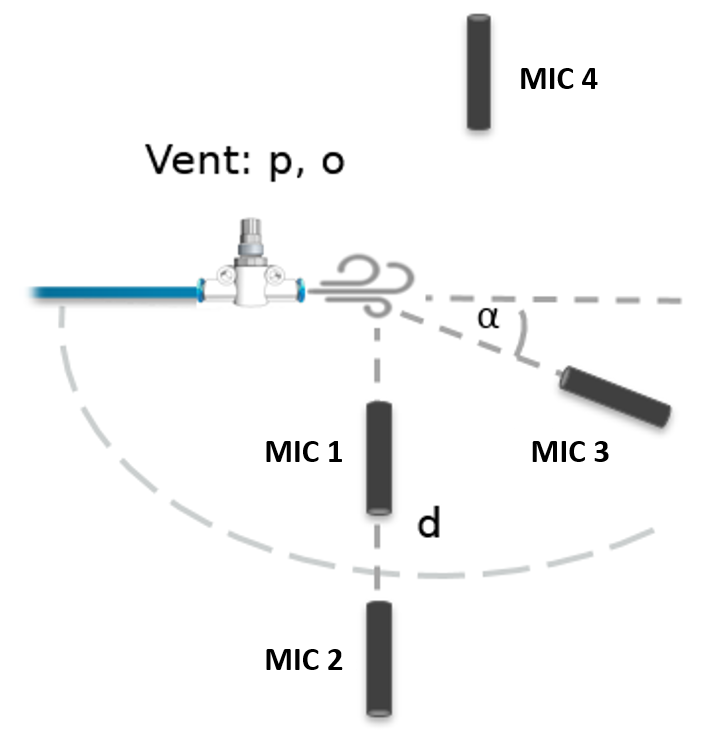
\includegraphics[clip,width=1\textwidth]{images/mic_positions.png}%
        \end{minipage}
    }
    \subfloat[]{
        \centering%
        \begin{minipage}[c][1\width]{0.48\textwidth}%
            \begin{center}
            \begin{tabular}{l l l} \toprule
                Mic & Distance ($d$) & Angle ($\alpha$)\\ \midrule
                1 & 20 cm & 90°\\
                2 & 2 m & 90°\\
                3 & 20 cm & 30°\\
                4 & Full Room & -\\ \bottomrule
            \end{tabular}
            \par
            \end{center}%
        \end{minipage}
    }
    \caption{Microphone position}
    \label{fig:mic_pos}
\end{figure}

To record acoustic emissions in the audible range, Earthworks M30 omnidirectional measurement microphones\footnote{\url{https://earthworksaudio.com/products/microphones/measurement-series/m30/}} with a frequency response in the range 3 Hz to 30 kHz are employed to record sound generated by the experimental apparatus described in Section \ref{sec:dataset}.\ref{subsec:app}.  % HACK FOR NOW
To evaluate the influence of microphone placement on leak detection, the microphones are positioned in four different locations with varying distances and angles, see Figure \ref{fig:mic_pos}. Three of the microphones (microphones 1-3) were oriented towards the leak source with an angle, $\alpha$ and distance, $d$, both described in Figure \ref{fig:mic_pos}, while the fourth microphone was placed in the center of the room near the ceiling to capture an ambient recording of the entire environment without direction.

\section{Compressed Air Leakage Dataset}\label{sec:dataset}

Using the experimental system described in Section \ref{sec:dataset}, we simulate and record a variety of conditions common to compressed air networks, including varying leak types, pressure levels and background noise. The normal pressure of the compressed air system is set to 6 bar. At this pressure level, we simulate two leak types with different acoustic characteristics: a leak that occurs at the choke vent (labeled as \textit{vent leak} throughout the rest of the paper), and a leak that occurs when a damaged tubing is installed into the system (\textit{tube leak}). A third leak is created by reducing the system pressure to 5 bar and creating a leak at the choke vent (\textit{vent low}). This introduces a leak with a lower amount of turbulence.

\begin{figure}[h]
	\centering
	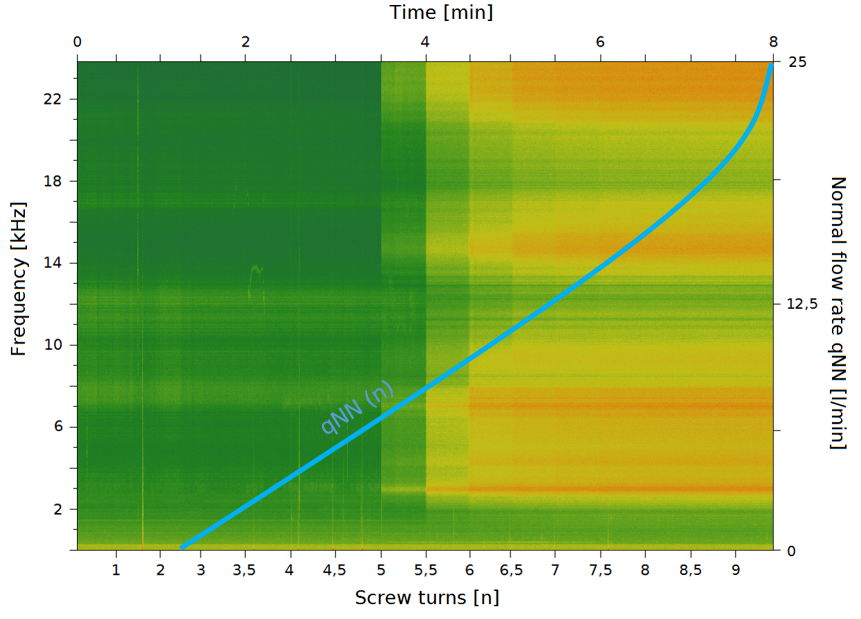
\includegraphics[width=88mm]{images/V_1_normi_qnn.png}
	\caption{Spectrogram of leakage noise from microphone position 1 with characteristic vent flow rate.}
	\label{fig:spec+qnn}
\end{figure}

To simulate normal and leak states, the amount of air escaping from the a choke vent is controlled using a knob which opens and closes the vent. Each successive turn of the knob opens the vent further, causing air to leak out. For the first three knob states, the knob is turned a complete rotation, after that the knob is turned in half rotations for each state. This is done for zero to nine turns resulting in 16 knob states. From 0 to 3 turns no air leaks from the system, and we consider these to be a non-leak states. From 3.5 to 5 turns, there is a minor leak, but the noise is not captured with our microphones, see Figure \ref{fig:spec+qnn}. In the signals recorded at 5.5 to 9 turns there is an audible acoustic emission, and this data is labeled as a leak state. 

Additionally, to mimic real-world conditions of production facilities, during recording sessions the compressed air system is recorded with one of three types of background noise. The first one is the laboratory environment noise which is introduced by the recording room itself, and contains minimal noise artefacts (called \textit{lab} throughout the rest of the paper). The other two types of noise are real-world factory noise recordings, including a typical workshop noise (\textit{workshop}, or \textit{work}) that contains aperiodic, diffuse noises, and a periodic, bolting and creaking sound created by a large hydraulic piston (\textit{hydraulic}, or \textit{hydr}). These noises are introduced into the data by playing the noise recordings on speakers in the laboratory during recording sessions. For each noise type, sessions are recorded with the noise playback at a high volume as well as low volume (indicated in the results by appending noise type with \textit{low}), which is set at 50\% of the high volume. This combination of environmental parameters results in fifteen system configurations, which can be seen in Table \ref{tab:noise-train}. Spectrograms showing the frequency content of the signals from the different leaks with the varying background noises, are shown in Figure \ref{fig:specs}. 

\begin{figure}[h]
	\centering
	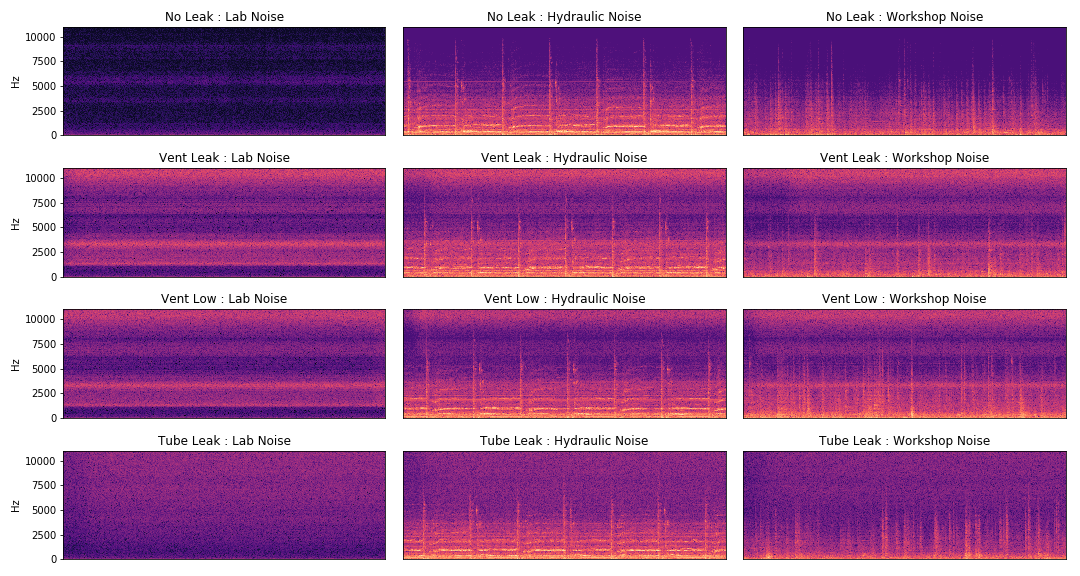
\includegraphics[width=0.95\columnwidth]{images/specs.png}
	\caption{Spectrograms from example recordings for each leak and background noise type. All data is from microphone 1.}
	\label{fig:specs}
\end{figure}

To limit bias in our data and to obtain valid results, we perform three recording sessions in which each of the 15 configurations were recorded. For each session, all four microphones are recording to ensure the data from each microphone is comparable. During the sessions, we record for 30 seconds at each each knob setting, resulting in 240 seconds of no leak recordings and 240 seconds of recordings with the specified leak for each microphone\footnote{The data from one of the sessions for the condition \textit{vent leak, workshop low} was corrupted and is not included in the full data. We mark this condition with an * in the results.}.

% \newpage